\documentclass[11pt,a4paper,twocolumn]{IEEEtran}
\usepackage[utf8]{inputenc}
\usepackage{tabularx, booktabs}
\usepackage{amsmath}
\usepackage{amsfonts}
\usepackage{caption}
\usepackage{pdfpages}
\usepackage[margin=2.5cm]{geometry}
\usepackage{listings}
\usepackage{amssymb}
\usepackage{hyperref}
\usepackage{graphicx}
\usepackage{svg}

\usepackage{biblatex}
\addbibresource{bib3.bib}

\newcolumntype{L}[1]{>{\raggedright\let\newline\\\arraybackslash\hspace{0pt}}m{#1}}
\newcolumntype{C}[1]{>{\centering\let\newline\\\arraybackslash\hspace{0pt}}m{#1}}
\newcolumntype{R}[1]{>{\raggedleft\let\newline\\\arraybackslash\hspace{0pt}}m{#1}}

% \sepline dopo \maketitle rende tutto più carino
\newcommand{\sepline}{\noindent\makebox[\linewidth]{\rule{\textwidth}{1.2pt}}}
\newcommand{\bsepline}{\noindent\makebox[\linewidth]{\rule{7.5cm}{1.2pt}}}
%\newcommand{\esepline}{\noindent\makebox[\linewidth]{\rule{7.5cm}{0.5pt}}}
\newcommand{\thinsepline}{\noindent\makebox[\linewidth]{\rule{7.5cm}{0.02pt}}}
\newcommand{\thinnersepline}{\noindent\makebox[\linewidth]{\rule{7.5cm}{0.01pt}}}

\author{Monaco Saverio - 2012264 \sepline \\Neural Networks and Deep Learning - Professor: A. Testolin}
\title{{\normalsize\textsc{Università degli studi di Padova}}\vspace{-.5cm} \\ \sepline\\ \textbf{Homework \#3
\\ Deep Reinforcement Learning}}

\begin{document}
	\maketitle
	\begin{abstract} The final homework concerns Deep-Q Learning, an algorithm of Deep Reinforcement Learning based on \textit{Bellman equation} for decision processes.\\
	Two environments of OpenAI Gym are tested with the algorithm: "CartPole-v1" where a 2-dimensional platform must balance straight a pole, and a custom environment of the popular mobile game "FlappyBird".\\
	For the latter, two different state-space encodings are probed: a smaller space that employs only 2 numerical variables, and a bigger encoding that contains the game visual output.
	\end{abstract}
    \section*{\textbf{Deep-Q Learning}}
    Deep-Q Learning is algorithm that belongs to the class of Deep Learning problems of Reinforcement Learning.
    In this branch of Deep Learning, an agent can interact with the surrounding environment (simulated or real). By the resulting states it is possible to give the agent a reward, namely a parameter that it tries to maximize.\\
    The goal of this algorithm is to find an optimal \textit{policy}, namely a rule that outputs the action to make, given the state of the system. The way to determine the \textit{policy function} is not unique, Deep-Q Learning relies on the \textit{Bellman equation} with the hypothesis that every instance is a Markov Process.\medskip\\
    For both environments, two optimizations are implemented to the vanilla algorithm:
    \begin{itemize}
		\item \textit{Experience Replay:} The agent does not learn while it acts on the environment. It follows the last policy for an arbitrary number of episodes, then it updates its policy computing the loss, sampling from its past [state, action] pairs. This helps the convergence of the algorithm by having a more i.i.d-like data samples.
		\item \textit{Target Network:} Two similar networks are implemented for a more stable update rule
	\end{itemize}
	A final note about Deep-Q Learning theory regards the \textit{Exploitation vs. Exploration} problem, namely wether to choose to follow the current policy to get the most reward, or to perform non-optimal actions according to the current policy in order for the agent to improve its knowledge about actions with more long term benefits. For the training of all the following models, a parameter called "T" (temperature) was implemented, the higher T is, the more exploration is performed. This parameter is gradually decreased during training using an exponential rule.
	% explain deep q learning
	\section{\textbf{CartPole-v1}}
		% explain game
		The first environment taken into consideration is "CartPole-v1". It consists in a cart that can move on a 1-dimensional rail. At the centre of the cart, a pole is pinned to one of its end. The goal is to avoid the pole to fall by moving the cart left or right along the rail.
		\begin{figure}[h]
			\centering
			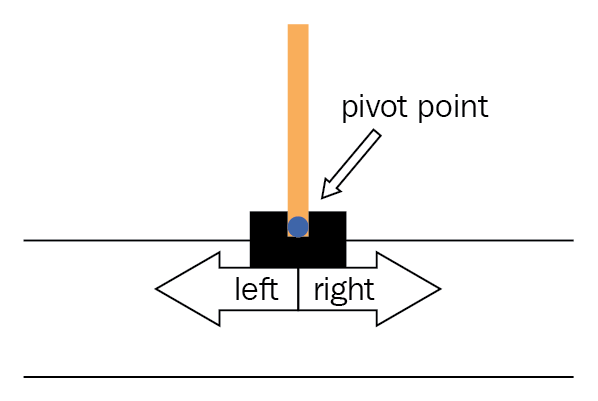
\includegraphics[width=0.75\linewidth]{../imgs/cartpole}
			\caption{CartPole-v1 graphical representation}
		\end{figure}
		\subsection{\textbf{Methods}}
		% describe your model architectures and hyperparameters
		For the CartPole environment the dimension of the observation space (namely the size of the state-vector that completely defines every state) is 4-dimensional \cite{GHCP}:
		\begin{itemize}
			\item Cart x-position: range = [-4.8, +4.8]
			\item Cart x-velocity: range = [-$\infty$,+$\infty$]
			\item Pole Angle: range $\sim$ [-24\textdegree , +24\textdegree]
			\item Pole Angular Velocity: range = [-$\infty$,+$\infty$]
		\end{itemize}
		The Cart can only either move left or right, the action space is then 2 dimensional.\medskip\\
		
		
		The Policy and Target networks are simple linear Networks:
		\begin{itemize}
			\item \textit{Input Layer}
			\begin{itemize}
				\item input\_size = 4 (state space dimension);
				\item output\_size = 128;
			\end{itemize}
			\item \textit{Hidden Layer}
			\begin{itemize}
				\item input\_size = 128
				\item output\_size = 128;
			\end{itemize}
			\item \textit{Output Layer}
			\begin{itemize}
				\item input\_size = 128
				\item output\_size = 2 (action space dimension);
			\end{itemize}
		\end{itemize}
		Between each layer, \texttt{nn.Tanh()} activation function was chosen.\medskip\\
		
		The goal was to find an optimal model that required the least amount of episodes as possible to learn how to balance the pole. For this reason, during the training of each model, after every update of the weights, the current network was tested on 10 games with 0 temperature, if it could balance the pole until the end (500 frames) on all games, the model was said
		to have learned.\medskip\\
		
		Various models were tested with different hyperparameters using Optuna, in the search of the model that could ace the 10 games with the least amount of learning as possible.
		\thinsepline\\
		\textbf{Parameters for Optuna Optimization:}\medskip\\
		\begin{tabular}{ll}
			Trials: & 30 \\
			Epochs: & 1000 \\
			\hline\vspace*{-.4cm}\\
			Regularization: & [1e-5, 1e-3] \\
			Lr: & [1e-4, 1e-3] \\
			Optimizer: & Adam, SGD\\
			Gamma: & [.95, 1]\\
			Initial T:& [1, 10]\\
		\end{tabular}\\
		\thinsepline\\
		\newpage
		\subsection{\textbf{Results}}\text{   }\\
		%  present the simulation results
		\thinsepline\\
		\textbf{Best parameters:}\medskip\\
		\begin{tabular}{ll}
			Regularization: & 0.0002 \\
			Lr: & 0.0003 \\
			Optimizer: & Adam \\
			Gamma: & 0.976 \\
			Initial T:& 2.107 \\
			\hline\\
			\multicolumn{2}{l}{Learned in 500 episodes}
		\end{tabular}\\
		\thinsepline\medskip\\
		During the training, the models spent a considerable portion of their initial episodes scoring very low values, having the agents no idea on what to do, but once the average score goes higher, they tended to score rapidly the maximum.
	% explain deep q learning
	\section{\textbf{FlappyBird}}
		% explain game
		Flappy Bird was a popular game for smartphone devices in the year 2014. In this game, the player must control the height of a bird by tapping on the screen, resulting in a flutter of its wings, while the bird's x-position is always fixed.\\ The game consists in avoiding incoming obstacle, namely vertical pipes that have a hole at a random height, in order to keep playing, the player must tap the screen accordingly to enter each pipe's hole, never touching the obstacles. This requires high level of precision for being the gaps narrow.\vspace*{-.2cm}
		\begin{figure}[h]
			\centering
			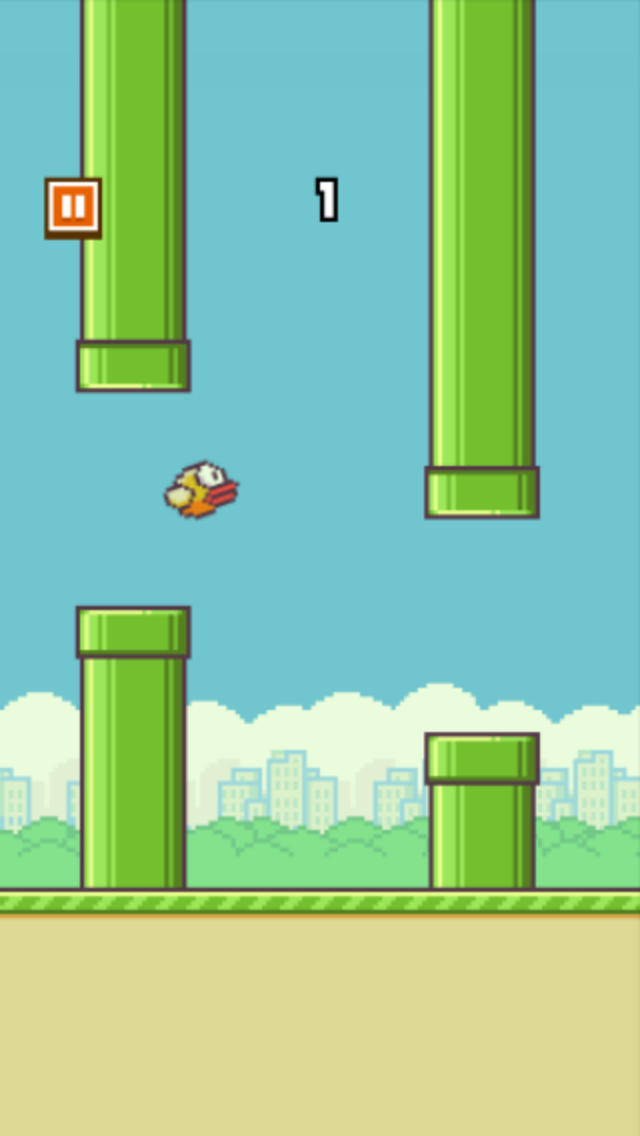
\includegraphics[width=0.35\linewidth]{../imgs/gameplay.jpeg}
			\caption{Gameplay example of the game}
		\end{figure}\vspace*{-1cm}\\
		\subsection{\textbf{FlappyBird-v0}}
			\subsubsection{\textbf{Methods}}
			% describe your model architectures and hyperparameters
			In this environment, the state-space is 2-dimensional:
			\begin{itemize}
				\item horizontal distance to the next pipe:\\ range = [-$\infty$,+$\infty$]
				\item difference between the player's y position and the next hole's y position:\\ range = [-$\infty$,+$\infty$]
			\end{itemize}
			While the possible actions are just two:
			\begin{itemize}
				\item Fly upwards (originally the tap of the screen): \texttt{action value = 1}
				\item Do nothing \texttt{action value = 0}
			\end{itemize}
		
			\begin{figure}[h]
				\centering
				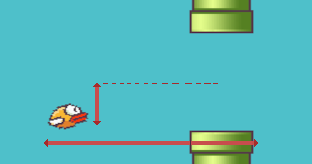
\includegraphics[width=0.75\linewidth]{../imgs/github1}
				\caption{State space of FlappyBird-v0 environment}
			\end{figure}
			Regarding the reward and punishes, the agent takes a point for every frame the game has not ended, and it gets a punishment proportionally to the vertical distance of the next hole. This punishment rule was mainly implemented to guide the agent for the first stages of learning, since without it would always fly way up (infact, if the policy is mostly random, the actions are equiprobable, however, fluttering the wings increases the y-position way more than doing nothing can decrease it, resulting in a general increase of the height before even encountering any obstacle).\medskip
		
			For this environment, the very same Policy and Target Networks class used for \texttt{CartPole-v1} were adopted.
			\thinsepline\\
			\textbf{Parameters for Optuna Optimization:}\medskip\\
			\begin{tabular}{ll}
				Trials: & 10 \\
				Epochs: & 1000 \\
				\hline\vspace*{-.4cm}\\
				Lr: & [1e-4, 1e-3] \\
				Optimizer: & Adam, SGD\\
				Gamma: & [.95, 1]\\
				Initial T:& [3, 6]\\
			\end{tabular}\\
			\thinsepline\\
			The best model was chosen by letting the agent play 10 times at the end of its training and choose the one with the highest mean score.\\
			\subsubsection{\textbf{Results}}\text{   }\\
			%  present the simulation results
			\thinsepline\\
			\textbf{Best parameters:}\medskip\\
			\begin{tabular}{ll}
				Lr: & 0.0004 \\
				Optimizer: & Adam \\
				Gamma: & 0.96 \\
				Initial T:& 5.34 \\
				\hline\\
				\multicolumn{2}{l}{Mean Score on Test Games: 2490 }
				
			\end{tabular}\\
			\thinsepline\medskip\\
			The model seems to be applied successfully in this environment aswell, however, the agent still loses each game eventually, mostly when sharp turns must be performed taking into account not only the incoming obstacle, but also the following one. However in this environment, the latter information is totally missing and a more extensive learning will not probably result in significative improvements of its executions. Nonetheless it has achieved a performance way above the average human player by usually surpassing the 70th-pipe.
		\subsection{\textbf{FlappyBird-rgb-v0}}
			The very same task was performed with the visual game output as state space.\\ Ideally, this new type of observation space could surpass the lack of information exposed for the environment before.
			
			\subsubsection{\textbf{Methods}}
			% describe your model architectures and hyperparameters
			State space was reduced through channel selections, maxpooling and cropping due to the long times required during the learning phase. See Appendix C for the state space optimization process.\\
			State space is:
			\begin{itemize}
				\item 14$\times$40 grayscale image
			\end{itemize}
			Possible actions are the same as before:
			\begin{itemize}
				\item Fly upwards (originally the tap of the screen): \texttt{action value = 1}
				\item Do nothing \texttt{action value = 0}
			\end{itemize}\vspace{.5cm}
			
			For the type of state the space data, a convolutional network for both the policy and target network was considered to be more fitting:
			\begin{itemize}
				\item \textit{First convolutional layer}
				\begin{itemize}
					\item in\_channels = 1;
					\item out\_channels = 8;
					\item kernel\_size = 5;
					\item stride = 2;
					\item padding = 1;
				\end{itemize} 
				\item \textit{Second convolutional layer}
				\begin{itemize}
					\item in\_channels = 8;
					\item out\_channels = 16;
					\item kernel\_size = 5;
					\item stride = 2;
					\item padding = 1;
				\end{itemize} 
				\item \textit{First linear layer}
				\begin{itemize}
					\item input\_size = 288
					\item output\_size = 64
				\end{itemize}
				\item \textit{Second linear layer}
				\begin{itemize}
					\item input\_size = 64
					\item output\_size = 2 (action space dimension)
				\end{itemize}
			\end{itemize}
			Between each layer, \texttt{nn.Tanh()} activation function was chosen.\medskip\\
			Due to the longer training times, the hyperparameters optimization was limited to just 5 trials:\\
			\thinsepline\\
			\textbf{Parameters for Optuna Optimization:}\medskip\\
			\begin{tabular}{ll}
				Trials: & 5 \\
				Epochs: & 1600 \\
				\hline\vspace*{-.4cm}\\
				Lr: & [1e-4, 1e-3] \\
				Optimizer: & Adam, SGD\\
				Gamma: & [.95, 1]\\
				Initial T:& [3, 6]\\
			\end{tabular}\\
			\thinsepline\\
			\subsubsection{\textbf{Results}}\text{   }\\
			%  present the simulation results
			\thinsepline\\
			\textbf{Best parameters:}\medskip\\
			\begin{tabular}{ll}
				Lr: & 0.0002 \\
				Optimizer: & Adam \\
				Gamma: & 0.973 \\
				Initial T:& 5.108 \\
				\hline\\
				\multicolumn{2}{l}{Mean Score on Test Games: 108.3 }
				
			\end{tabular}\\
			\thinsepline\medskip\\
			Although the performances are significantly lower with respect to the 2-dimensional state-space encoding, this model is still able to occasionally avoid the first obstacles, meaning that it was able to learn something from the compressed images.\\
			An extended hyperparameters search and longer training times would be without doubt beneficial to this model, however, the hyperparameters search was indentionally limited due to the exponentially longer training times with respect to the two previous environments treated.\medskip\\
			The best models for \textit{CartPole} and \textit{FlappyBird} were saved using \texttt{torch.save()} function. Two scripts were written that load these models as policy network and they are able to show how they play:
			\begin{itemize}
				\item[-] \texttt{qcartpole.py} to see an attempt in the CartPole-v1 environment;
				\item[-] \texttt{qflappy.py} to see the agent play a Flappy Bird game;
			\end{itemize}
			For the latter, the package \texttt{flappy-bird-gym} must be installed\cite{GHFB}:
			$$\text{\texttt{\$ pip install flappy-bird-gym}}$$
			\newpage
			Additionally, two videos were uploded on Youtube showing the average performance:
			\begin{itemize}
				\item \href{https://www.youtube.com/watch?v=LSkuY9bjZlo}{CartPole-v1 video}
				\item \href{https://www.youtube.com/watch?v=QKapLxaR-3Q&t=14s}{FlappyBird-v0 video}
			\end{itemize} 
			
			%  present the simulation results
			\nocite{brockman2016openai}
			\nocite{mnih2013playing}
			\printbibliography
	\newpage
	\onecolumn
	\section{\textbf{Appendix}}
		\subsection{\textbf{CartPole-v1 hyperparameter optimization}}
		\begin{figure}[h]
			\centering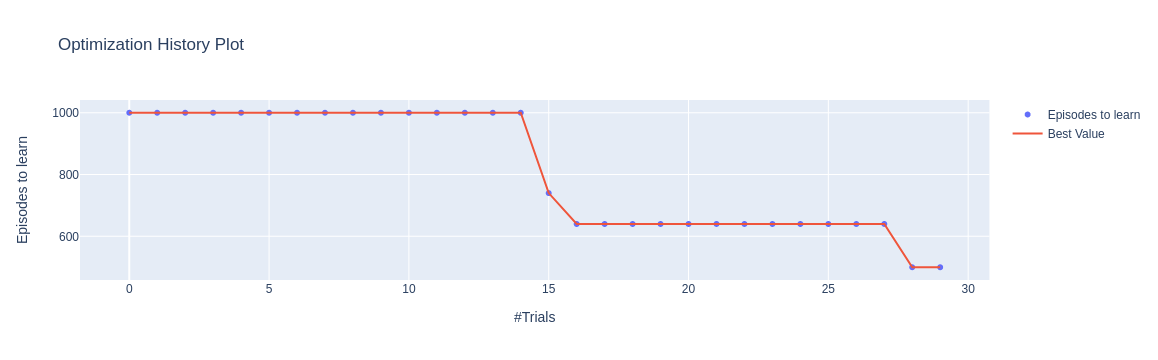
\includegraphics[width=1\linewidth]{../imgs/optuna_cartpole}\vspace*{-.7cm}
			\caption{Hyperparameter optimization of CartPoe-v1 environment in Optuna}
			\label{fig:cartpoleopt}
		\end{figure}
		During the training of each model, every 10 episodes their policies were tested in 10 games with T=0. The best model was chosen by finding the one that takes the least amount of episodes to score 500 on all the 10 games with zero temperature.\medskip\\
		The search of the best parameters was further optimized by interrupting the learning of all the models that were taking longer, with respect to the best model found to date, to reach the above requirement, that is the reason why the curve of the figure \ref{fig:cartpoleopt} is not-increasing.
		\subsection{\textbf{FlappyBird-v0 hyperparameters optimization}}\vspace*{-.5cm}
		\begin{figure}[h]
			\centering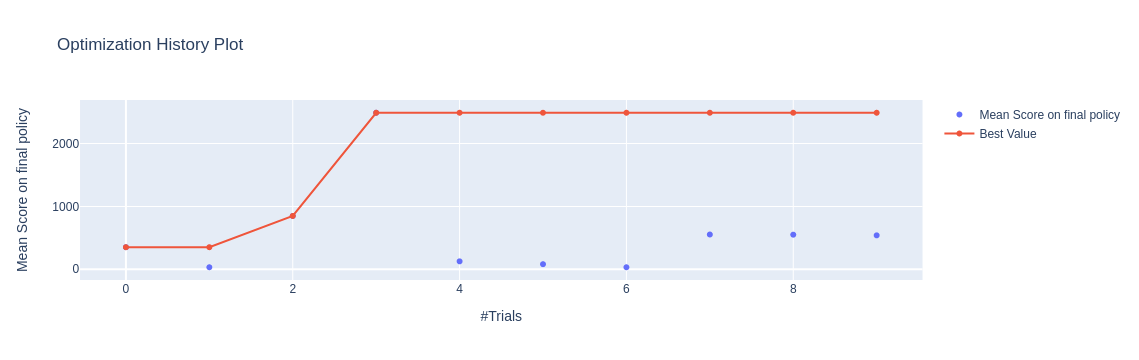
\includegraphics[width=1\linewidth]{../imgs/optuna_fbv0_1}\vspace*{-.7cm}
			\caption{Final Mean Scores of FlappyBird-v0 models}
			\label{fig:fbv01opt}
		\end{figure}
	\begin{figure}[h]
		\centering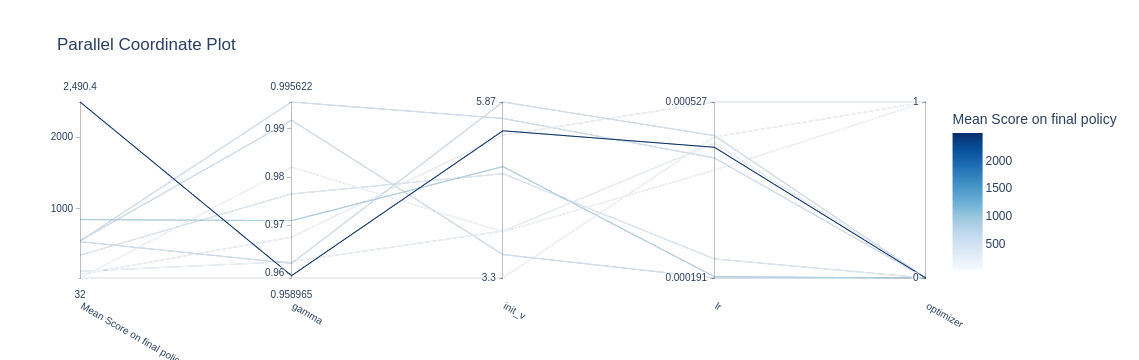
\includegraphics[width=1\linewidth]{../imgs/optuna_fbv0_2}\vspace*{-.0cm}
		\caption{Hyperparameter optimization of CartPoe-v1 environment in Optuna}
		\label{fig:fbv02opt}
	\end{figure}
		\newpage
		\subsection{\textbf{Coordinate Plot of FlappyBird-v0 hyperparameters}}
		\label{section:aprgb}
		For the environment FlappyBird-rgb-v0, the original state space corresponds to the game visual output with a screen size of 288$\times$512, the dimension of the state space is then 288$\times$512$\times$3, that is 442,368.\vspace*{-1cm}\\
		\begin{figure}[h]
			\centering
			\includesvg[width=0.65\linewidth]{../imgs/default_view}\vspace*{-.7cm}
			\caption{Original example of State space of FlappyBird-rgb-v0 environment}
		\end{figure}\\
		For curiosity, this encoding of the state space was tested, resulting in several seconds for every time the function \texttt{update\_step()} was called. Considering the large amount of time it would take to train the model enough epochs with this state space encoding, the process was killed and optimizations were considered.\medskip\\
		
		\subsubsection{Single channel image} The first obvious optimization is to choose a single channel from the whole RGB image, reducing the size of the state space by a factor of 3. Additionally, there are two main areas that contains no visual information, namely the bottom area where the ground is, and the area left to the agent, hence the screen was cropped removing them.\\ This reduced the size of the state space from 442,368 to 84,000.\vspace*{-1cm}\\
		\begin{figure}[h]
			\centering
			\includesvg[width=0.65\linewidth]{../imgs/single_channel_cropped}\vspace*{-.7cm}
			\caption{Single channel (Green) and Cropped}
		\end{figure}
		\newpage
		\subsubsection{Lowering resolution} The major advandage was obtained by maxpooling the state image, lowering its resolutiong. The maximum kernel size (10) was applied to obtain the highest gain in training time, bringing the dimension of the state space from 84,000 down to 840.\vspace*{-1cm}\\
		\begin{figure}[h]
			\centering
			\includesvg[width=0.75\linewidth]{../imgs/single_channel_cropped_maxpooled10}\vspace*{-1cm}
			\caption{Maxpooled (10)}
		\end{figure}
		\subsubsection{Further pooling of right side of the screen} With the idea that the attention of the agent should be channeled mostly to the incoming obstacle, the right side of the screen was maxpooled horizontally, merging horizontally the pixels among the ones in the blue area and in the red area of the figure, further lowering the state space dimensionfrom 840 to 560.\vspace*{-1cm}\\
		\begin{figure}[h]
			\centering
			\includesvg[width=0.75\linewidth]{../imgs/single_channel_cropped_maxpooled10_reduced}\vspace*{-1cm}
			\caption{Horizontal pooling of right (distant) pixels}
		\end{figure}\newpage
		In the following figure the original and final state space encodings are shown for a direct comparison. All the size reduction of the state space caused a loss of information that can cause the model to converge slower (or not at all), however, it seems that all the essential information are still kept in the reduced encoding.\vspace*{-1cm}\\
		\begin{figure}[h]
			\centering
			\includesvg[width=0.75\linewidth]{../imgs/original_to_reduced}\vspace*{-1cm}
			\caption{Full state-space transformation}
		\end{figure}\\
		\textbf{Total improvement:} 442,368 $\to$ 560
\end{document}